\section{Solution}

In this section we propose the approaches with centralized coordination.
\begin{enumerate}
\item The first strategy, mentioned above, is the \srst which consider only 
one task allocated for one robot.

\item The second strategy (\gsp) extends the first, the main concept of this strategy 
is merging the tasks with greedy approach. 

\item The last strategy \sps extends the second algorithm using a optimize merging tasks. 
\end{enumerate}

\subsection{Single robot : Single task (\srst)}

This method is a baseline for our logistic scenario.
The important constraint of this approach is consider only one task allocated for 
one robot at time.
Given a set of tasks, the \texttt{task\_planner} assigns only one task at time,
if the robot request a task.
\\
The set of tasks is ordered by the function mentioned below.
\begin{lstlisting}
inline bool pop_min_element(const Task &A, const Task &B) {
    if ((A.dst < B.dst) && (A.demand < B.demand)) {
      return 1;
    } else if (A.dst == B.dst) {
      return 1;
    }
    return 0;
  }
\end{lstlisting}
Such function sort the tasks based on the distance of the unloading bays and the demand of a specific task.

The \texttt{task\_planner} post-processing all task, compute the route by a sequence 
of vertices, and the cost of the path. After having assigned the task $t_{i,j}$ 
it is deleted.

\subsection{Greedy Set Partition Strategy Single robot : Multiple task (\gsp)}

The main concept of this approach is merging tasks using Greedy Coalition Formation
based on \cite{cf_greedy} and \cite{cf_farinelli}. Where one wants to minimize the 
team cost subject to the constraint that each task must be executed by a given 
number of cooperative agents simultaneosly. Each task requires a number of different 
demands, and each coalition for the task needs to provide the requered capabilities.

For compute coalition the heuristic is based on the concept of Gain, which can be 
defined for any pair of coalitions $C_i$, $C_j$ as:
\[G(C_i,C_j) = v(\{C_i \cup C_j\}) - v(C_i) - v(C_j)\]
where $v(C)$ is value of the characteristic function $v$ for coalition $C$. 
In other words, this gain function captures the value of synergies between coalitions
and is computed in constant time.

The function $v$ for a coalition $C_i$ is defined as:
\[ v(C_i) = \frac{|\pi_i|}{|demand_i|}\]
where $|\pi_i|$ is the path distance between the loading bay $L$ and the unloading bays $U_j$
and the $|demand_i|$ is the demand of the task.

The same function for a pair of coalition $C_i$, $C_j$ can be defined as:
\[  v(\{C_i \cup C_j\}) = \frac{|\pi_i|}{|demand_i|} + \frac{|\pi_j|}{|demand_j|} = \sum_{i,j} \frac{|\pi_{i,j}|}{|demand_{i,j}|} \]

We want minimize the cost of the gain, that can be defined as:
\[G(C_i,C_j) < 0 \]
if the gain $G$ is less than 0 then we allocate the pair and delete the element which
form the coalition.

The core of this algorithm is reported below as pseudocode.
\begin{algorithm}
    \caption{Greedy Coalition Formation}\label{GSF}
    % \begin{algorithmic}[1]
        % Initialize partitions to singletons
    $T = {{t_0},{t_1}, \cdots, {t_N}}$
    % \end{algorithmic}
\end{algorithm}

\subsection{Set Partition Strategy Single robot : Multiple task (\sps)}

This method consists to compute all possible coalitions of the task set and use only 
the best coalition which is based on the previously mentioned heuristic $v$.

\subsection*{Example with 9 tasks and 4 robots}
Given a set of tasks $T = {{{t_0},{t_1}, \cdots, {t_9}}}$ defined like: 
${t_i=(item, demand, unloading\_bay)}$. The agents have the same capacity $C_{0,1,2,3} = 4$.

For \textbf{example}:
\newline
$T=\{t_0(A,1,U_0), t_1(B,1,U_1), t_2(C,1,U_2), t_3(A,2,U_0), t_4(B,2,U_1),t_5(C,2,U_2), t_6(A,3,U_0), t_7(B,3,U_1), t_8(C,3,U_2)\}$

The result of the Greedy Coalition Formation is:
\newline
$T'= \{ t_5(C,2,U_2), t_6(A,3,U_0),t_7(B,3,U_1),t_8 (C,3,U_2),t_{\{2,4\}}(\{C,B\},3,U_{1,2}), t_{\{0,1,3\}}(\{A,B\},4,U_{0,1}) \}$

\begin{figure} [hbt]
    \centering
    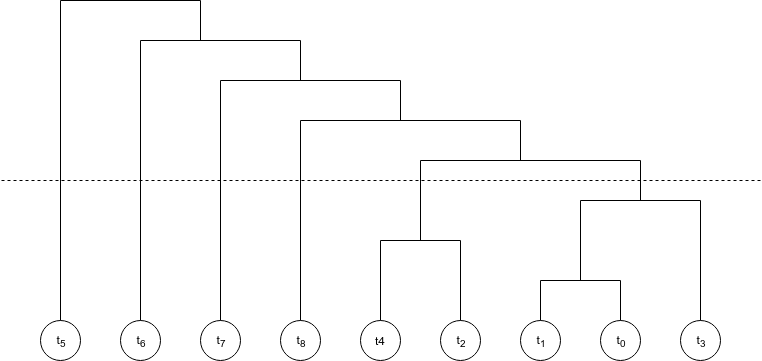
\includegraphics[width=\textwidth]{img/CF_graph.png}
    \caption{An exemplar dedrogram representing a possible hierarchical
    clusterung for 9 tasks. The horizontal line represents a cut of the dendrogram
    and defines the coalition structure
    $\{ t_5(C,2,U_2), t_6(A,3,U_0),t_7(B,3,U_1),t_8 (C,3,U_2),t_{\{2,4\}}(\{C,B\},3,U_{1,2}), t_{\{0,1,3\}}(\{A,B\},4,U_{0,1}) \}$.}
    \label{fig:CF_graph}
\end{figure}




